\section{绪论}\label{sec:introduction}

LaTeX(通常发音为 "Lay-tech" 或 "Lah-tech")是一种高质量排版系统,它特别适用于技术和科学文档的制作。LaTeX 基于 TeX 排版系统,由 Donald Knuth 开发,而 LaTeX 本身则是由 Leslie Lamport 在20世纪80年代创建的。LaTeX 的主要特点包括:

\begin{enumerate}
    \item \textbf{高度专业的排版质量:} LaTeX 能够生成极为专业和美观的文档,特别是对数学公式和科学文档的处理。
    \item \textbf{内容与样式分离:} 用户主要关注内容的输入,而文档的格式和样式由 LaTeX 的内部算法处理,确保了文档的一致性和专业性。
    \item \textbf{广泛的定制和扩展性:} 通过不同的宏包(packages),LaTeX 可以用于生成各种类型的文档,如学术论文、书籍、幻灯片等。
    \item \textbf{强大的数学公式支持:} LaTeX 提供了丰富的数学符号和公式排版功能,这也是其在学术界广泛使用的主要原因。
    \item \textbf{跨平台:} LaTeX 可以在多种操作系统上运行,如 Windows、Mac OS 和各种 Linux 系统。
    \item \textbf{开源免费:} LaTeX 是免费软件,用户可以自由使用和修改。
\end{enumerate}

虽然 LaTeX 拥有许多优点,但它也有一定的学习曲线。在下面的章节中,我们将介绍如何使用 LaTeX 撰写毕业设计论文。我们将从安装 LaTeX 开始,然后介绍如何使用 LaTeX 撰写文档,最后介绍如何使用本模板。

\section{安装 LaTeX}

各个平台的安装方法不同,我们将分别介绍 Windows、Mac OS 和 Linux 系统下的安装方法。

\subsection{Windows}

对于 Windows 用户,我们推荐使用TeX Live。TeX Live 是一个跨平台的 TeX 发行版,它包含了大量的宏包和工具,可以满足大多数用户的需求。

TeX Live 有两种安装方式:网络安装和镜像安装。网络安装需要联网,它会从网络上下载安装文件,因此安装过程会比较慢。镜像安装则不需要联网,它会从本地镜像文件安装,因此安装过程会比较快。我们推荐使用镜像安装,因为它不仅安装速度快,而且可以避免网络问题导致的安装失败。TeX Live 的镜像文件可以从\href{https://mirrors.ustc.edu.cn/CTAN/systems/texlive/Images/}{中科大开源镜像站}下载。我们推荐下载 \texttt{texlive.iso},它是一个 ISO 镜像文件,可以使用 Windows 自带的虚拟光驱软件直接挂载并安装。如果你不知道如何挂载 ISO 镜像文件,请自行搜索。

\subsection{MacOS}

对于 MacOS 用户,我们推荐使用 MacTeX。MacTeX 是一个专门为 MacOS 用户准备的 TeX 发行版,它和 TeX Live 是同一个项目的不同版本,两者除了名字不同外,其他都是一样的。MacTeX 的安装方式和 TeX Live 一样,也有网络安装和镜像安装两种方式。我们推荐使用镜像安装,因为它不仅安装速度快,而且可以避免网络问题导致的安装失败。MacTeX 的镜像文件可以从\href{https://mirrors.ustc.edu.cn/CTAN/systems/mac/mactex/}{中科大开源镜像站}下载。我们推荐下载 \texttt{MacTeX.pkg},它是一个 pkg 安装包,可以直接双击安装。

\subsection{Linux}

对于 Linux 用户,我们同样推荐使用 TeX Live,并且两者的镜像文件是相同的,都可以从\href{https://mirrors.ustc.edu.cn/CTAN/systems/texlive/Images/}{中科大开源镜像站}下载。此外,在 Linux 下 还可以使用命令行进行安装,只需要在挂载镜像后在目录下执行 \texttt{sudo ./install-tl} 命令即可。当然,在基于 Debian 的 Linux 发行版(如 Ubuntu)下,也可以使用 \texttt{sudo apt-get install texlive-full} 命令进行安装,但是这种方式安装的 TeX Live 版本较旧,不推荐使用。

\section{LaTeX 编辑器}

LaTeX 是一种标记语言,它的源文件是纯文本格式,因此可以使用任何文本编辑器进行编辑。由于本人主要使用 Visual Studio Code,因此本教程主要介绍如何在 Visual Studio Code 中使用 LaTeX,其他编辑器只进行简单的介绍。

\subsection{TeXstudio}

TeXstudio 是一款跨平台的 LaTeX 编辑器,它是 TeXmaker 的一个分支,提供了丰富的功能,如语法高亮、智能补全、编译预览等。TeXstudio 的安装包可以从\href{https://www.texstudio.org/}{官网}下载,一般来说该软件会随着 TeX Live 的安装一并安装到系统中。

\begin{figure}[htb!]
    \centering
    \begin{subfigure}{.3\textwidth}
        \centering
        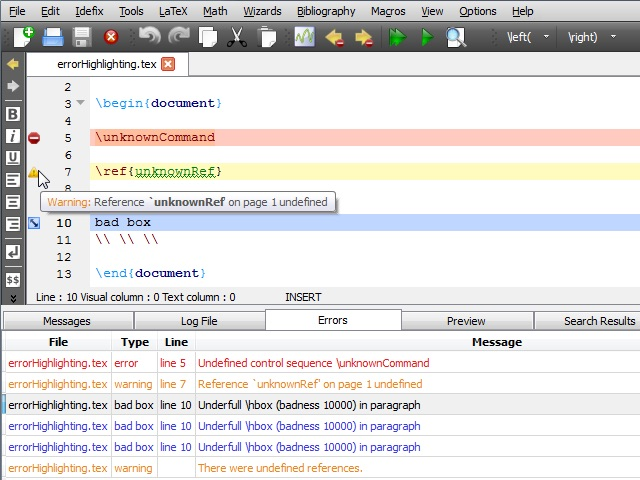
\includegraphics[width=.9\textwidth]{./img/texstudio1.jpeg}
        \caption{错误提示}
        \label{fig_texstudio_1}
    \end{subfigure}
    \begin{subfigure}{.3\textwidth}
        \centering
        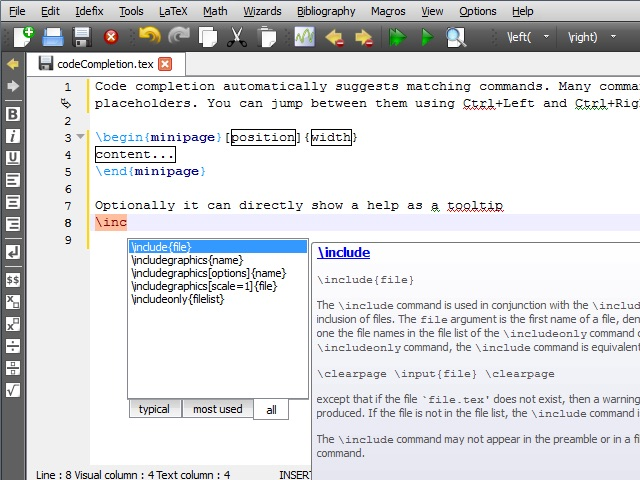
\includegraphics[width=.9\textwidth]{./img/texstudio2.jpeg}
        \caption{代码补全}
        \label{fig_texstudio_2}
    \end{subfigure}
    \begin{subfigure}{.3\textwidth}
        \centering
        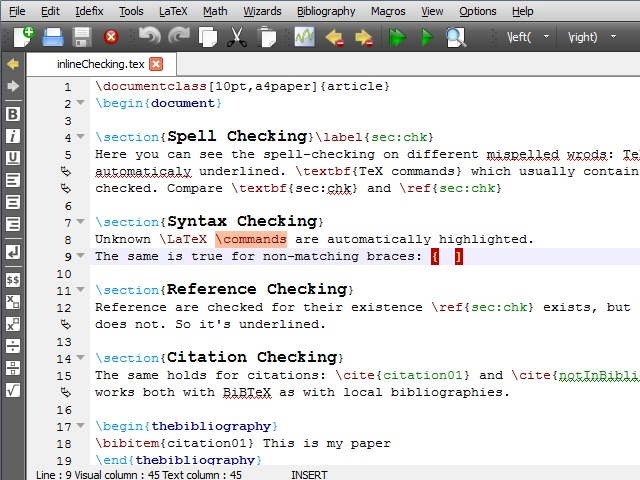
\includegraphics[width=.9\textwidth]{./img/texstudio3.jpeg}
        \caption{代码检查}
        \label{fig_texstudio_3}
    \end{subfigure}
    \caption{TeXstudio 界面展示}
    \label{fig_texstudio}
\end{figure}

\subsection{Visual Studio Code}

Visual Studio Code 是一款跨平台的轻量级代码编辑器,它支持多种编程语言,如 C/C++、Python、Java、JavaScript 等。最值得一提的是,Visual Studio Code 有着丰富的插件生态系统,用户可以根据自己的需求安装各种插件,从而实现各种功能,比如 LaTeX Workshop 这个插件针对 LaTeX 提供了丰富的功能:语法高亮、智能补全、编译预览等,Visual Studio Code 的安装包可以从\href{https://code.visualstudio.com/}{官网}下载。

至于如何在 Visual Studio Code 中配置 LaTeX 环境,本人早已写过一份教程,感兴趣的同学可以参考\href{https://github.com/shinyypig/latex-vscode-config}{这里}。该教程中搭建的环境支持如下功能:

\begin{enumerate}
    \item 保存文件时自动编译
    \item 支持 XeLaTeX 和 PdfLaTeX 编译 (中英文)
    \item 编译结果输出到特定文件夹./tmp
    \item 英文单词补全,以及中文翻译
    \item LaTeX 语法自动补全
    \item 支持快速输入公式,比如输入@a会自动补全为\textbackslash alpha
    \item 自动补全路径
    \item 自动生成矩阵和图片环境
    \item 实时预览公式、图片
    \item 自动格式化 tex 文件
\end{enumerate}

再加上如今语言模型的支持,编写 LaTeX 文档将会变得更加轻松。

\begin{figure}[htb!]
    \centering
    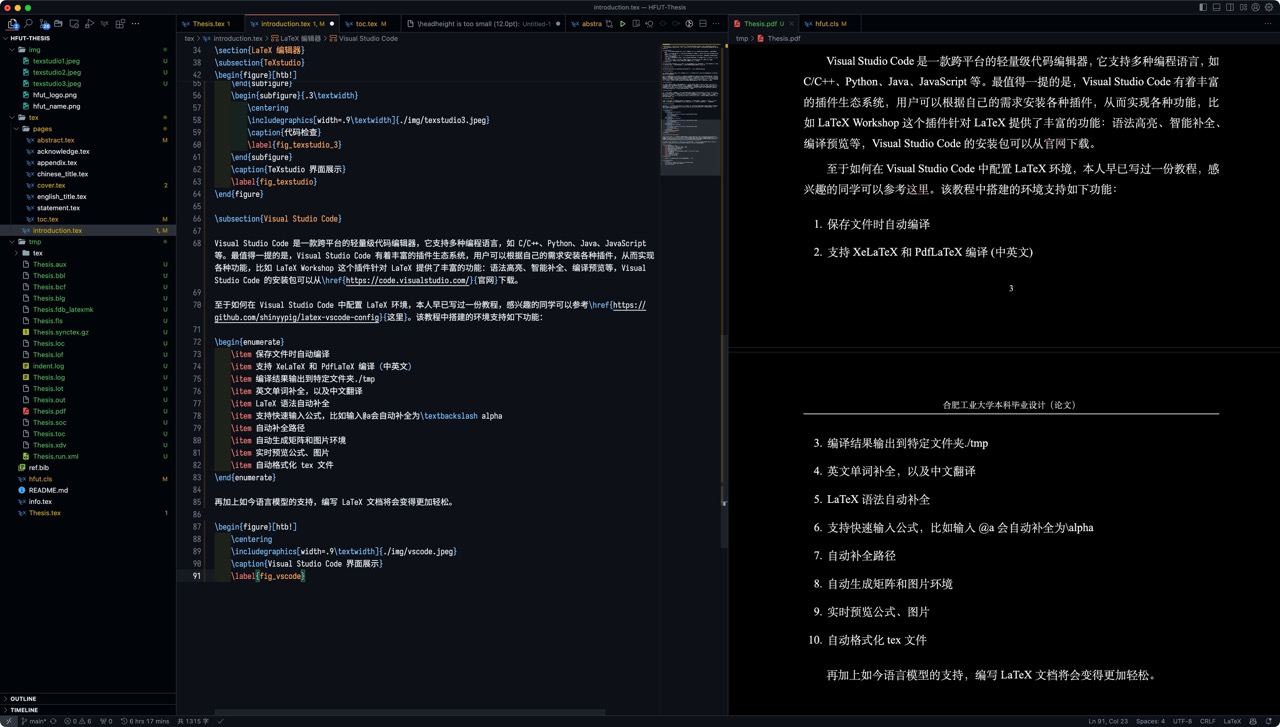
\includegraphics[width=.9\textwidth]{./img/vscode.jpeg}
    \caption{Visual Studio Code 界面展示}
    \label{fig_vscode}
\end{figure}

\section{编写 LaTeX 文档}

本小节将介绍如何使用 LaTeX 编写文档,包括一些基本知识,以及如何插入公式、插入图片、插入表格、插入参考文献等。

\subsection{章节和段落}

在 LaTeX 中,我们可以使用 \texttt{\textbackslash section}、\texttt{\textbackslash subsection} 和 \texttt{\textbackslash subsubsection} 命令来创建章节。比如,本小节标题对应的代码为 

\begin{lstlisting}[language=TeX]
\subsection{章节和段落}
\end{lstlisting}

此外,在 LaTeX 中换行并不会产生新的段落,如果需要新的段落,我们需要在段落之间插入一个空行,即

\begin{lstlisting}[language=TeX]
这是第一个段落。

这是第二个段落。
\end{lstlisting}

\noindent 会生成如下效果:

这是第一个段落。

这是第二个段落。

你可以使用 \% 符号来注释掉一行内容,比如

\begin{lstlisting}[language=TeX]
% 这是一行注释
这是一行正文。
\end{lstlisting}

\noindent 会生成如下效果:

% 这是一行注释
这是一行正文。

可以看到,注释掉的内容不会被编译。

\subsection{公式}
在 LaTeX 中,我们可以使用 \texttt{\textbackslash (} 和 \texttt{\textbackslash )} 命令来创建一个行内公式,比如

\begin{lstlisting}[language=TeX]
著名的欧拉公式 \(e^{i\pi} = -1\) 是数学中最美丽的公式之一。
\end{lstlisting}

\noindent 会生成如下效果:

著名的欧拉公式 \(e^{i\pi} = -1\) 是数学中最美丽的公式之一。


我们可以使用 \texttt{\textbackslash begin\{equation\}} 和 \texttt{\textbackslash end\{equation\}} 命令来创建一个带有编号的公式,比如

\begin{lstlisting}[language=TeX]
\begin{equation}
    \sum_{i=1}^{n} i = \frac{n(n+1)}{2}.
\end{equation}
\end{lstlisting}

\noindent 会生成如下效果:

\begin{equation}
    \sum_{i=1}^{n} i = \frac{n(n+1)}{2}.
\end{equation}

如果不需要编号,我们可以使用 \texttt{\textbackslash [} 和 \texttt{\textbackslash ]} 命令来创建一个不带编号的公式,比如

\begin{lstlisting}[language=TeX]
\[ 
    \sum_{i=1}^{n} i = \frac{n(n+1)}{2}.
\]
\end{lstlisting}

\noindent 会生成如下效果:

\[ 
    \sum_{i=1}^{n} i = \frac{n(n+1)}{2}.
\]

我们可以使用 \texttt{\textbackslash begin\{aligned\}} 和 \texttt{\textbackslash end\{aligned\}} 命令来创建一个带有多行的公式,比如

\begin{lstlisting}[language=TeX]
\begin{equation}
    \begin{aligned}
        a & = b + c  \\ 
        d & = e + f + g
    \end{aligned}
\end{equation}
\end{lstlisting}

\noindent 会生成如下效果:

\begin{equation}
    \begin{aligned}
        a & = b + c      \\ 
        d & = e + f + g
    \end{aligned}.
\end{equation}
其中,\texttt{\&} 用于对齐,\texttt{\textbackslash\textbackslash} 用于换行。

还可以使用 \texttt{\textbackslash begin\{matrix\}} 和 \texttt{\textbackslash end\{matrix\}} 命令来创建一个矩阵,比如

\begin{lstlisting}[language=TeX]
\begin{equation}
    \begin{bmatrix}
        1 & 2 & 3 \\
        4 & 5 & 6 \\
        7 & 8 & 9
    \end{bmatrix}
\end{equation}
\end{lstlisting}

\noindent 会生成如下效果:

\begin{equation}
    \begin{bmatrix}
        1 & 2 & 3  \\
        4 & 5 & 6  \\
        7 & 8 & 9
    \end{bmatrix}
\end{equation}

更多的公式用法同学们可以根据自己的需求自行搜索。

\subsection{图片}

在 LaTeX 中,我们可以使用 \texttt{\textbackslash includegraphics} 命令来插入图片,比如

\begin{lstlisting}[language=TeX]
\begin{figure}[htb!]
    \centering
    
\includegraphics[width=.9\textwidth]{img/eg1.png}
    \caption{示例图片1}
    \label{fig_eg1}
\end{figure}
\end{lstlisting}

\noindent 会生成如下效果:

\begin{figure}[htb!]
    \centering
    
\includegraphics[width=.4\textwidth]{img/eg1.png}
    \caption{示例图片1}
    \label{fig_eg1}
\end{figure}

其中,\texttt{[htb!]} 用于设置图片的位置,\texttt{h} 表示将图片放在当前位置,\texttt{t} 表示将图片放在页面顶部,\texttt{b} 表示将图片放在页面底部,\texttt{!} 表示忽略一些限制。如果不设置图片位置,LaTeX 会自动选择一个合适的位置放置图片,一般来说推荐使用\texttt{htb!}。此外,\texttt{\textbackslash centering} 命令用于将图片居中,\texttt{\textbackslash caption} 命令用于设置图片标题,\texttt{\textbackslash label} 命令用于设置图片标签。\texttt{width=.4\textbackslash textwidth} 表示将图片的宽度设置为当前页面宽度的 0.4 倍,当然你也可以设置图像的高度,比如 \texttt{height=.4\textbackslash textwidth}。最后,\texttt{img/eg1.png} 表示图片的路径。通常,LaTeX 支持的图片格式有 \texttt{.png}、\texttt{.jpg}、\texttt{.pdf} 等。

如果需要插入多张图片,我们可以使用 \texttt{\textbackslash begin\{subfigure\}} 和 \texttt{\textbackslash end\{subfigure\}} 命令来插入子图,比如

\begin{lstlisting}[language=TeX]
\begin{figure}[htb!]
    \centering
    \begin{subfigure}{.4\textwidth}
        \centering
        
\includegraphics[height=.15\textheight]{./img/cat1.jpeg}
        \caption{小猫1}
        \label{fig_cat_1}
    \end{subfigure}
    \begin{subfigure}{.25\textwidth}
        \centering
        
\includegraphics[height=.15\textheight]{./img/cat2.jpeg}
        \caption{小猫2}
        \label{fig_cat_2}
    \end{subfigure}
    \begin{subfigure}{.25\textwidth}
        \centering
        
\includegraphics[height=.15\textheight]{./img/cat3.jpeg}
        \caption{小猫3}
        \label{fig_cat_3}
    \end{subfigure}
    \caption{示例图片2}
    \label{fig_cat}
\end{figure}
\end{lstlisting}

\noindent 会生成如下效果:

\begin{figure}[htb!]
    \centering
    \begin{subfigure}{.4\textwidth}
        \centering
        
\includegraphics[height=.15\textheight]{./img/cat1.jpeg}
        \caption{小猫1}
        \label{fig_cat_1}
    \end{subfigure}
    \begin{subfigure}{.25\textwidth}
        \centering
        
\includegraphics[height=.15\textheight]{./img/cat2.jpeg}
        \caption{小猫2}
        \label{fig_cat_2}
    \end{subfigure}
    \begin{subfigure}{.25\textwidth}
        \centering
        
\includegraphics[height=.15\textheight]{./img/cat3.jpeg}
        \caption{小猫3}
        \label{fig_cat_3}
    \end{subfigure}
    \caption{示例图片2}
    \label{fig_cat}
\end{figure}

从中我们可以看到,\texttt{\textbackslash begin\{subfigure\}} 和 \texttt{\textbackslash end\{subfigure\}} 命令用于创建子图,\texttt{\textbackslash caption} 命令用于设置子图标题,\texttt{\textbackslash label} 命令用于设置子图标签,\texttt{.4\textbackslash textwidth} 表示子图的宽度为当前页面宽度的 0.4 倍,\texttt{.15\textbackslash textwidth} 表示子图的高度为当前页面高度的 0.15 倍。

\subsection{表格}

在 LaTeX 中,我们可以使用 \texttt{\textbackslash begin\{tabular\}} 和 \texttt{\textbackslash end\{tabular\}} 命令来创建一个表格,比如

\begin{lstlisting}[language=TeX]
\begin{table}[htb!]
    \centering
    \begin{tabular}{|c|c|c|}
        \hline
        1 & 2 & 3 \\
        \hline
        4 & 5 & 6 \\
        \hline
        7 & 8 & 9 \\
        \hline
    \end{tabular}
    \caption{示例表格}
    \label{tab_eg}
\end{table}
\end{lstlisting}

\noindent 会生成如下效果:

\begin{table}[htb!]
    \centering
    \begin{tabular}{|c|c|c|}
        \hline
        1 & 2 & 3 \\
        \hline
        4 & 5 & 6 \\
        \hline
        7 & 8 & 9 \\
        \hline
    \end{tabular}
    \caption{示例表格}
    \label{tab_eg}
\end{table}

推荐使用 \href{https://www.tablesgenerator.com/}{Tables Generator} 可视化编辑表格,并生成对应的 LaTeX 代码。

\subsection{伪代码}

在 LaTeX 中,我们可以使用 \texttt{\textbackslash begin\{algorithm\}} 和 \texttt{\textbackslash end\{algorithm\}} 命令来创建一个伪代码,比如

\begin{lstlisting}[language=TeX]
\begin{algorithm}[htb!]
    \caption{示例伪代码}
    \label{alg_eg}
    \begin{algorithmic}[1]
        \REQUIRE $n \geq 0$
        \ENSURE $y = x^n$
        \STATE $y \gets 1$
        \STATE $X \gets x$
        \STATE $N \gets n$
        \WHILE{$N \neq 0$}
            \IF{$N$ is even}
                \STATE $X \gets X \times X$
                \STATE $N \gets N / 2$
            \ELSE[$N$ is odd]
                \STATE $y \gets y \times X$
                \STATE $N \gets N - 1$
            \ENDIF
        \ENDWHILE
    \end{algorithmic}
\end{algorithm}
\end{lstlisting}

\noindent 会生成如下效果:

\begin{algorithm}[htb!]
    \caption{示例伪代码}
    \label{alg_eg}
    \begin{algorithmic}[1]
        \REQUIRE $n \geq 0$
        \ENSURE $y = x^n$
        \STATE $y \gets 1$
        \STATE $X \gets x$
        \STATE $N \gets n$
        \WHILE{$N \neq 0$}
        \IF{$N$ is even}
        \STATE $X \gets X \times X$
        \STATE $N \gets N / 2$
        \ELSE[$N$ is odd]
        \STATE $y \gets y \times X$
        \STATE $N \gets N - 1$
        \ENDIF
        \ENDWHILE
    \end{algorithmic}
\end{algorithm}

其中,\texttt{\textbackslash caption} 命令用于设置伪代码标题,\texttt{\textbackslash label} 命令用于设置伪代码标签,\texttt{\textbackslash REQUIER} 命令用于设置输入,\texttt{\textbackslash ENSURE} 命令用于设置输出,\texttt{\textbackslash STATE} 命令用于设置状态,\texttt{\textbackslash WHILE} 命令用于设置循环,\texttt{\textbackslash IF} 命令用于设置条件,\texttt{\textbackslash ELSE} 命令用于设置否定条件,\texttt{\textbackslash ENDWHILE} 命令用于结束循环,\texttt{\textbackslash ENDIF} 命令用于结束条件。

\subsection{引用}

在 LaTeX 中,我们可以使用 \texttt{\textbackslash label} 命令来设置标签,使用 \texttt{\textbackslash ref} 命令来引用标签,比如

\begin{lstlisting}[language=TeX]
\begin{equation}\label{eq_eg}
    \sum_{i=1}^{n} i = \frac{n(n+1)}{2}.
\end{equation}
式(\ref{eq_eg}) 是一个示例公式。
\end{lstlisting}

\noindent 会生成如下效果:

\begin{equation}\label{eq_eg}
    \sum_{i=1}^{n} i = \frac{n(n+1)}{2}.
\end{equation}
式(\ref{eq_eg}) 是一个示例公式。

不过,本模版内置了\texttt{cleveref}宏包,因此我们可以使用 \texttt{\textbackslash cref} 命令来引用标签,并且会自动识别标签的类型,比如

\begin{lstlisting}[language=TeX]
\begin{equation}\label{eq_eg2}
    \int_{-\infty}^{+\infty} e^{-x^2} dx = \sqrt{\pi}.
\end{equation}
\cref{eq_eg2} 是一个示例公式。
\end{lstlisting}

\begin{equation}\label{eq_eg2}
    \int \frac{1}{x^2} dx = -\frac{1}{x}.
\end{equation}
\cref{eq_eg2} 是一个示例公式。

类似地,我们可以引用图片,表格,伪代码等,比如

\begin{lstlisting}[language=TeX]
这是\cref{fig_eg1},这是\cref{tab_eg},这是\cref{alg_eg}。
\end{lstlisting}

这是\cref{fig_eg1},这是\cref{tab_eg},这是\cref{alg_eg}。

我们还可以一次性引用多个标签,比如

\begin{lstlisting}[language=TeX]
这些是\cref{fig_cat_1,fig_cat_2,fig_cat_3},那些是\cref{fig_eg1,tab_eg,alg_eg}。
\end{lstlisting}

这些是\cref{fig_cat_1,fig_cat_2,fig_cat_3},那些是\cref{fig_eg1,tab_eg,alg_eg}。

\subsection{参考文献}

在 LaTeX 中,我们可以使用 \texttt{\textbackslash cite} 或 \texttt{\textbackslash supercite} 命令来引用参考文献,比如

\begin{lstlisting}[language=TeX]
这是一个示例参考文献\cite{hfut-thesis},而这是一个上标形式的引用\supercite{hfut-thesis}。
\end{lstlisting}

这是一个示例参考文献\cite{hfut-thesis},而这是一个上标形式的引用\supercite{hfut-thesis}。

当然,类似于\texttt{\textbackslash cref},我们也可以一次性引用多个参考文献。所有的参考文献都保存在主目录的\texttt{ref.bib}文件中,如果需要添加参考文献,只需要在该文件中添加即可。一般来说,我们可以在 Google Scholar 中找到对应的参考文献,然后点击引用,选择 BibTeX 格式,复制粘贴到\texttt{ref.bib}文件中即可,其格式如下:

\begin{lstlisting}[language=TeX]
@article{hfut-thesis,
    author    = {Liangliang},
    journal   = {LaTeX Template},
    publisher = {Github},
    title     = {HFUT Thesis Template based on LaTeX},
    url       = {https://github.com/shinyypig/HFUT-Thesis},
    year      = {2023}
}
\end{lstlisting}

\section{使用本模板}

本模版需使用 XeLaTeX 编译,如果你使用的是 Visual Studio Code,并按照我的教程配置了 LaTeX 环境,那么只需保存即可编译,编译结果会输出到\texttt{./tmp}文件夹下。如果你使用的是其他编辑器,那么你需要自行配置编译环境。或者使用本项目提供的\texttt{build.bat} (windows) 和\texttt{build.sh} (linux\&mac) 进行编译。

使用本模版的同学首先要修改\texttt{info.tex}文件,将里面的信息修改为自己的信息,并完善\texttt{tex/pages}文件夹中的文件,包括摘要、致谢、附录等。如果需要添加新的章节,只需要在\texttt{tex}文件夹下添加对应的\texttt{.tex}文件,并在\texttt{Thesis.tex}中引入即可。

本模版还提供了两种不同的编译模式,方便同学们和导师之间沟通,分别是\texttt{preprint}模式和\texttt{final}模式。其中,\texttt{preprint}模式下会在文档左侧显示行号,方便沟通时定位问题,并且在这个模式下导师批阅的内容也会显示出来,方便修改。使用的是\texttt{changes}宏包,有需求的老师可自行学习相关用法,非常简单。

而\texttt{final}模式下则不会显示行号,也不会显示导师批阅的内容,这是最终的打印版本。默认情况下,本模版使用\texttt{final}模式,如果需要切换到\texttt{final}模式,只需要在\texttt{Thesis.tex}中将\texttt{mode}设置为\texttt{final}即可,如下所示:

\begin{lstlisting}[language=TeX]
% final 模式
\documentclass{hfut}
% preprint 模式
\documentclass[mode=preprint]{hfut}
% final 模式
\documentclass[mode=final]{hfut}
\end{lstlisting}